\chapter{Implementation}

\section{Problem Statement}

This case study aims on to make the inversion of a single element feedforward neural network. However the implementation of the inversion is just the last step during the process, because the dataset needs a lot of preprocessing to make the predictable model.\smallskip

This work belongs in the realm of machine learning application research. There are three main tasks examinated in this paper: data mining for extracting information from a data set, building and testing multilayer perceptron models for, and inverting these feedforward neural network models. \medskip

The first task is to choose a dataset which contains predictable data. The selected dataset is called the Online News Popularity Dataset by Mashable news, that was served by the  \href{http://archive.ics.uci.edu/ml/datasets/Online+News+Popularity}{UCI's Machine Learning Repository}. \smallskip

The dataset is preprocessed for data mining by Pandas. Since being a publicly available dataset, its preprocessing and transformation has already done, but the dataset still needs some cleaning with the assistance of Scikit-Learn. The dataset contains a lot of outlying values that should be handled. Furthermore the dataset has a wide range of values, which necessitates a standard scaling. Then the dataset can be split into training and testing sets by Scikit-Learn. \medskip

The training phase consists of the application of machine learning techniques \cite{karayiannis2013artificial}. Different multi-layer perceptron models are fitted on the training set with various parameters. These attributes have iterated over different their hidden layer sizes, activation functions, optimization algorithms, learning rate sizes and alpha values. After Scikit-Learn trains the dataset and makes predictions to the testing set. The training is time consuming, since the used dataset is large and the length depends on the amount of attributes of multi-layer perceptron models. At the end of each process, the testing set's output and the predicted output are compared and the difference between them is calculated. If all of the iterations are over, the best estimator's parameters are shown with the score, and the tested target values and the predicted values are plotted by Matplotlib.\medskip

Now the main task, inversion can be executed. To perform the WLK inversion, the equations which are mentioned in \autoref{para:wlk-inv} have to be implemented \cite{nazari1992implementation}. The inversion is defined as a python function to be callable in the main program. In the inversion function, the network is initialized with a random input vector. Output is calculated and compared with the given output. Now the error can be calculated and backpropagated to minimize the loss function and the input vector has updated too. This iterative process continues until the error is less than the minimum set value. The return value is the guessed input value. \smallskip

At the end, the given testing set's values and the guessed input values are written to a .txt file with the accuracy percent of the inversion. A summarization about the accuracy percent values are described.



\subsection{Used Third-Party Libraries}

Python can be used effectively with the assistance of some of its third-party libraries \cite{bressert2012scipy}\cite{chen2017pandas}, which provide numerous effective and easy-to-use models in scientific research. \bigskip

\textbf{Pandas} is an open source library providing high-performance, easy-to-use data structures and data analysis tools for Python. Pandas has a main object called DataFrame, that is for data manipulation using a set of labeled array data structures. Pandas has tools for reading tabular data and writing data between in-memory data structures and different file formats. The data can be handled integratedly and the data sets are transformable. Some of the examples of this transformation are column insertion and deleting, data set merging and joining, or the hierarchical axis indexing in high-dimensional data models.\bigskip


\textbf{Matplotlib} is an open source Python library that produces publication-quality plots and figures. It ships with several add-on toolkits, including 3d plotting and assistance for axes. There are several common approaches of plotting in Matplotlib. The most popular is $pyplot$, which is a collection of command style functions where each $pyplot$ function makes some change to a figure. Also it is mainly intended for interactive plots and simple cases of programmatic plot generation.\bigskip

\textbf{NumPy} is a library for Python focused on multi-dimensional arrays and matrices. It provides high-level mathematical functions to operate on these arrays. In NumPy, the n-dimensional array is called $ndarray$, where all the elements of a single array must contain the same type. \medskip

\noindent The most important attributes of an $ndarray$ object are:\\
- $ndarray.ndim$ produces the number of axes of the array.\\
- $ndarray.shape$ produces the dimensions of the array.\\
- $ndarray.size$ is the total number of elements of the array.\\
- $ndarray.dtype$ is an object describing the type of the elements in the array.\\
- $ndarray.itemsize$ produces the size in bytes of each element of the array.\\
- $ndarray.data$ is a buffer, which contains the actual elements of the array.


\subsubsection{Scikit-Learn}

The most important package that is used during the implementation is Scikit-Learn \cite{Pedregosa2011ScikitlearnML}. It is a separately-developed and distributed third-party extension to SciPy. It integrates classic machine learning algorithms into the scientific Python packages. \smallskip

Scikit-Learn can be used to solve multi-layer neural network learning problems. Among many others, it features various classification, regression and clustering algorithms. Scikit-Learn contains all the various functions which can be used during the training of the neural network. The training lasts from the processing of the data set, via the iterations, to the inversion itself. \bigskip

\textbf{StandardScaler} is a subclass of Scikit-Learn's prepropressing class that standardizes features by removing the mean and scaling to unit variance. It has three parameters that are boolean values and the default of all is True: \smallskip

\noindent - $copy$ means if the original dataset will be replaced with the scaled one or not\\
- $with\char`_mean$ means if the scaler centers the data before scaling or not\\
- $with\char`_std$ means if the data is scaled to unit variance or not \medskip

The standard score of a sample $x$ is calculated as: $z = \frac{(x - u)}{s}$ where $u$ is the mean of the training samples or zero if $with\char`_mean=False$, and $s$ is the standard deviation of the training samples or one if $with\char`_std=False$. \medskip

\noindent StandardScaler has some methods:
\begin{verse}
	$\bullet$ $fit(X[, y])$ computes the mean and the standard deviation to be used for later scaling\\
	$\bullet$ $fit\char`_transform(X[, y])$ fits to data, then transforms it\\
	$\bullet$ $get\char`_params([deep])$ gets parameters for this estimator\\
	$\bullet$ $inverse\char`_transform(X[, copy])$ scales back the data to the original representation\\
	$\bullet$ $partial\char`_fit(X[, y])$ is the online computation of mean and standard deviation on $X$ for later scaling\\
	$\bullet$ $set\char`_params(**params)$ sets the parameters of this estimator\\
	$\bullet$ $transform(X[, y, copy])$ performs standardization by centering and scaling
\end{verse}\smallskip

\textbf{Train\char`_test\char`_split} is a subclass of Scikit Learn's selection class, which splits arrays or matrices into random train and test subsets. The randomization is important in ordered data sets. Allowed inputs are lists, NumPy arrays, SciPy-sparse matrices or Pandas DataFrames. Train\char`_test\char`_split returns with four lists that contains the train-test splits of inputs.\medskip

\noindent The parameters are the following:\smallskip

\noindent - $test\char`_size$ : If $float$, it should be between 0.0 and 1.0 and represents the proportion of the dataset to include in the test split. If $int$, it represents the absolute number of test samples. If $None$, the value is set to the complement of the train size. \\
- $train\char`_size$ : If $float$, it should be between 0.0 and 1.0 and represents the proportion of the dataset to include in the train split. If $int$, it represents the absolute number of train samples. If $None$, the value is automatically set to the complement of the test size.\\
- $random\char`_state$ : If $int$, it is the seed used by the random number generator. If $RandomState$ instance, it is the random number generator. If $None$, the random number generator is the $RandomState$ instance used by $np.random$.\\
- $shuffle$ : Whether or not to shuffle the data before splitting.\\
- $stratify$ : It shows if the data is split in a stratified fashion, using this as the class labels.\bigskip


\textbf{MLPRegressor} \cite{bengfort2018applied} is a class of Scikit-Learn, which implements a multi-layer perceptron, that uses the square error as the loss function. It trains iteratively because the partial derivatives of the loss function are computed in each step to update the parameters of the layers. MLPRegressor also supports multi-output regression, in which a sample can have more than one target outputs.\medskip

\noindent MLPRegressor has several parameters, but only a few of them will be listed, which were used in the implementation:
\begin{verse}
	$\bullet$ $hidden\char`_layer\char`_sizes$ is a tuple where the $i$th element represents the number of neurons in the ith hidden layer.
	
	$\bullet$ $activation$ is the activation function for the hidden layer.\\
	\hspace{10pt} - ‘identity’ provides the linear function, returns $f(x) = x$\\
	\hspace{10pt} - ‘logistic’ provides the logistic sigmoid function, returns $f(x) = \frac{1}{1 + e^{-x}}.$\\
	\hspace{10pt} - ‘relu’ provides the rectified linear unit function, returns $f(x) = max(0, x)$. \\
	\hspace{10pt} - ‘tanh’ provides the hyperbolic tan function, returns $f(x) = tanh(x)$.
	
	$\bullet solver$ is the optimization algorithm used in weight optimization.\\
	\hspace{10pt} - ‘sgd’ refers to stochastic gradient descent.\\
	\hspace{10pt} - ‘adam’ refers to a transition between adaptive methods and momentum-based methods.\\
	\hspace{10pt} - ‘lbfgs’ is an optimizer in the family of quasi-Newton methods.
	
	$\bullet alpha$ is the L2 regularization parameter's value.
	
	$\bullet learning\char`_rate\char`_init$ is the initial learning rate that is used. It controls the step-size in updating the weights. Only used when the solver is $sgd$ or $adam$.
	
	$\bullet learning\char`_rate$ means the learning rate schedule for weight updates. \\
	\hspace{10pt} - ‘constant’ is a constant learning rate given by $learning\char`_rate\char`_init$.\\
	\hspace{10pt} - ‘invscaling’ gradually decreases the learning rate at each time step using an inverse scaling exponent.\\
	\hspace{10pt} - ‘adaptive’ keeps the learning rate constant as long as training loss keeps decreasing.
\end{verse}
MLPRegressor contains built-in methods to perform regression:\\
- $fit(X, y)$ fits the model to data matrix $X$ and target(s) $y$.\\
- $get\char`_params([deep])$ gets parameters for this estimator.\\
- $predict(X)$ predicts an output based on previous training and a given testing dataset.\\
- $score(X, y[, sample\char`_weight])$ returns with the coefficient of the determinated prediction.\\
- $set\char`_params(^{**} params)$ sets the parameters of the estimator.\bigskip


\textbf{GridSearchCV} \cite{jolly2018machine} is an exhaustive searching class of Scikit-Learn over specified parameter values for an estimator. It can be used in the tuning of the hyper-parameters, which are those parameters that are not directly learnt within estimators. The parameters of the estimator used to apply the methods of GridSearchCV are optimized by cross-validated grid-search over a parameter grid.\medskip

\noindent The parameters of GridSearchCV are quite wide, but only a few of them are used during the implementation:
\begin{verse}
	$\bullet estimator$ implements the estimator interface. \\
	$\bullet param\char`_grid$ is a dictionary with the names of the used parameters as keys and lists of parameter settings to try as values.\\
	$\bullet cv$ is an integer that determines the cross-validation splitting strategy.\\
	$\bullet n\char`_jobs$ stands for the number of jobs to run in parallel. -1 means that the search uses all of the processors. 
\end{verse}

From GridSearchCV's attributes, $best\char`_params\char`_$ is used, which is a dictionary about the parameter setting that gave the best results on the hold out data.\medskip

\noindent GridSearchCV contains built-in methods for prediction:\\
- $fit(X[, y, groups])$ method fits with the adjusted parameter grid on the given dataset.\\
- $get\char`_params([deep])$ gets parameters for this estimator.\\
- $predict(X)$, $predict\char`_log\char`_proba(X)$ and $predict\char`_proba(X)$ make the prediction on the test set\\
- $score(X[, y])$ returns the score on the given data, if the estimator has been refit.\\
- $set\char`_params(**params)$ sets the parameters of this estimator.\bigskip


\section{The Implementation}

The first step was to import all of the necessary libraries.
\begin{lstlisting}
import numpy as np
import pandas as pd
import matplotlib.pyplot as plt
from sklearn.neural_network import MLPRegressor
from sklearn.preprocessing import StandardScaler
from sklearn.model_selection import train_test_split
from sklearn.model_selection import GridSearchCV
import inversion
\end{lstlisting}
The $inversion$ library is not a built-in library of Python, it is importing the written function from another .py file.\smallskip

After, the selected dataset has captured by Pandas. In this case the used dataset is a .csv file, which contains 39.644 instances and 61 attributes. The attributes consist of 58 predictive features, 2 other attributes of accessory information and 1 goal field, which is the number of shares. The dataset represents as a matrix, where the columns are the features and the rows are the data. This dataset is preprocessed by Pandas as a DataFrame object. The $url$ and $timedelta$ columns have been omitted, since they are meta-data and cannot be treated as features. 
\begin{lstlisting}
dataset = pd.read_csv('OnlineNewsPopularity.csv')
dataset_copy = dataset.drop(columns=['url','timedelta'])
\end{lstlisting}

\medskip As already mentioned, the dataset's preprocessing and transformation has done, but the dataset still needs cleaning. Before execute the cleaning phase, the summarization of the dataset needs a review to see the data that need to be cleaned.
\begin{lstlisting}
dataset_copy.describe()
\end{lstlisting}
where the first 5 columns results the following from the initial dataset:
\begin{figure}[h]
	\centering
	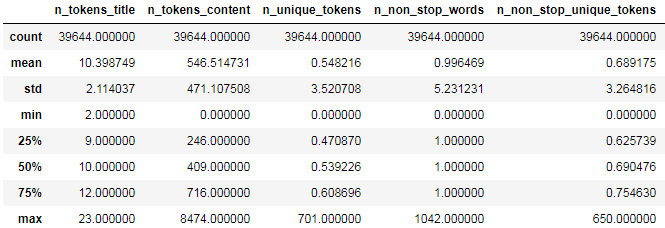
\includegraphics[height=0.34\linewidth]{./figures/describe1}
	\label{fig:describe1}
\end{figure}

\noindent As it can be seen in the table, there are outlying values that would cause noise if they are not handled. Also, in the known of the meaning of each columns, some inconsistencies are occured, like the $n\char`_tokens\char`_content$ feature contains the number of words in the content, which cannot be zero. These inconsistent values needs a correction.


\subsection{Optimizing the Dataset}

There are a lot of techniques in data mining for optimizing the data into appropriate forms. In the case of outlying and inconsistent values, due to the huge number of data, the chosen technique was to simply ignore those tuples. 
\begin{lstlisting}
dataset_copy = dataset_copy[dataset_copy.n_tokens_content != 0]
dataset_copy = dataset_copy[dataset_copy.n_unique_tokens <= 1]
dataset_copy = dataset_copy[dataset_copy.average_token_length != 0]

dataset_copy = dataset_copy[dataset_copy.num_hrefs <= 100]
dataset_copy = dataset_copy[dataset_copy.num_self_hrefs <= 10]
dataset_copy = dataset_copy[dataset_copy.num_imgs <= 10]
dataset_copy = dataset_copy[dataset_copy.num_videos <= 2]
dataset_copy = dataset_copy.reset_index(drop=True)
\end{lstlisting}

These reductions need some explanation. As mentioned above, $n\char`_tokens\char`_content$ is the number of words in the content, so it cannot be zero. $n\char`_unique\char`_tokens$ contains the rate of unique words in the content. Because of $n\char`_unique\char`_tokens$ is a rate, it need to be between [0,1]. The $average\char`_token\char`_length$ contains the average length of the words in the content, which also cannot be zero. \smallskip

The other optimizations are for handling the outlying values. $num\char`_hrefs$ contains the number of links, $num\char`_self\char`_hrefs$ is the number of links to other articles published by Mashable, $num\char`_imgs$ has the number of images and $num\char`_videos$ stands for the number of videos. Furthermore because this dataset is a Pandas DataFrame and $drop$ is a function for removing the whole row, the dataset needs to be reindexed.\medskip

After the cleaning, the dataset's other part is still has a big difference between its values, so the whole dataset should be scaled. 
\begin{lstlisting}
scaler = StandardScaler()
dataset_copy[:] = scaler.fit_transform(dataset_copy[:])
\end{lstlisting}
With the usage of StandardScaler's $fit\char`_transform$ method, the dataset has been fitted and transformed in one step. \medskip

\noindent Then the dataset has separated into feature $X$ and target $y$ groups.
\begin{lstlisting}
y = dataset_copy.pop('shares')
X = dataset_copy
\end{lstlisting}
The column $shares$ contains the target values, which are the number of shares.\medskip

Learning the parameters of a prediction function and testing the accuracy of the learning on the same data is a methodological mistake: a model that is just repeating the values of the samples, the model would have a perfect score, but it cannot predict anything useful from the data that are not seen yet. This situation is called overfitting. To avoid it, a common practice is when performing a supervised machine learning experiment to hold out a part of the available data as a testing set $X\char`_test$, $y\char`_test$. 
\begin{lstlisting}
X_train, X_test, y_train, y_test = train_test_split(X, y, test_size=0.3, random_state=0)
\end{lstlisting}
Now the training ($X\char`_train$, $X\char`_test$) and testing ($y\char`_train$, $y\char`_test$) sets are made. The $test\char`_size$ is a float, which means the testing sets have this proportion from the dataset.



\subsection{Training the Neural Network}

Then the dataset is ready to be trained. The training consists of the application of machine learning techniques. Different multi-layer perceptron models are fitted on the training sets with a set of parameters $param\char`_grid$. These parameters are the number of hidden layers, the activation functions, the optimization algorithms, the alpha value, the learning rate's type and the learning rate's initialize value. Scikit-Learn's training toolkit is called MLPRegressor, which is used as an estimator of GridSearchCV. The process of the training fits the neural network model to the training sets, then tests the accuracy on the testing sets by predicting the output $y\char`_pred$.  
\begin{lstlisting}
mlp = MLPRegressor()
param_grid = {
	'hidden_layer_sizes': [(3,10,3)],
	'activation': ['relu', 'logistic', 'tanh'],
	'solver': ['lbfgs', 'adam'],
	'alpha': [0.03, 0.01, 0.003, 0.001],
	'learning_rate_init': [0.03, 0.01, 0.003, 0.001],
	'learning_rate': ['adaptive'],
}
gs = GridSearchCV(mlp, param_grid, cv=2, n_jobs=-1)
gs.fit(X_train, y_train)
\end{lstlisting}
This process is time consuming due to the amount of the given parameters are trained on a large-scale dataset. The search was running on a supercomputer and  the training lasts for days. The score was computed by the L2 norm of the loss function, which means the difference between the original and the predicted value. \smallskip

It can be seen, that stochastic gradient descent is not on the list of the optimization methods. When the dataset was trained, SGD causes NaN or infinite values during the calculation of the gradients. The solution was to remove SGD from the solvers. \medskip

After the trained multi-layer perceptron is ready, the results can be stored and the received values can be plotted by Matplotlib.
\begin{lstlisting}
regressor = gs.best_estimator_
print(regressor, 'score: ', gs.best_score_, sep='\n ', file=open('TrainingResult.txt', 'w'))

y_pred = regressor.predict(X_test)

plt.plot(X_test, y_test, 'o', color='blue')
plt.plot(X_test, y_pred, 'o', color='orange')
plt.savefig('./' + 'prediction.pdf')
plt.show()
\end{lstlisting}
The results of the training contains a summarization of the best estimator and the score. It can be seen that the score was $0.018810289564545335$ and the best estimator parameters were the logistic activation function and L-BFGS as optimization algorithm, with the use of $0.03$ alpha value and $0.01$ initial learning rate. The training uses $3$ hidden layers with $(100,200,500)$ neurons in each layers.
\begin{lstlisting}
MLPRegressor(activation='logistic', alpha=0.03, batch_size='auto', 
	beta_1=0.9, beta_2=0.999, early_stopping=False, epsilon=1e-08, hidden_layer_sizes=(100, 200, 500), learning_rate='adaptive', learning_rate_init=0.01, max_iter=200, momentum=0.9, n_iter_no_change=10, nesterovs_momentum=True, power_t=0.5, random_state=None, shuffle=True, solver='lbfgs', tol=0.0001, validation_fraction=0.1, verbose=False, warm_start=False) 
score: 0.018810289564545335
\end{lstlisting}

\smallskip The results of the training are shown on the following \autoref{fig:shares}, where the original values are colored blue and the predicted ones have color orange:
\begin{figure}[h]
	\centering
	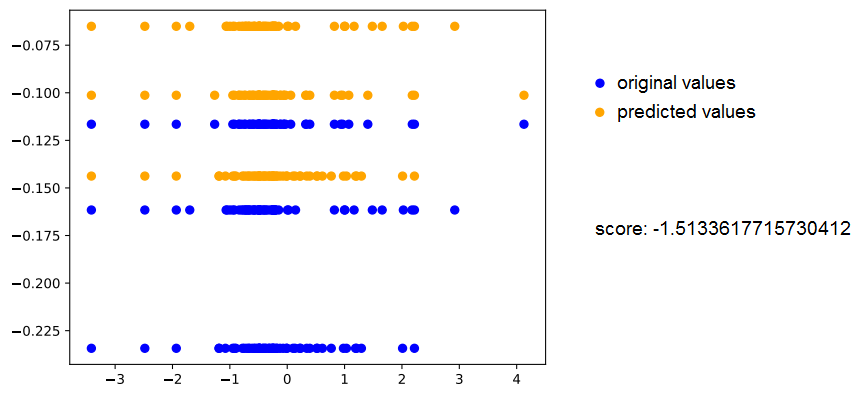
\includegraphics[height=0.38\linewidth]{./figures/prediction}
	\caption{The result of the best prediction}
	\label{fig:shares}
\end{figure}

\medskip It is a long process to train a multi-layer perceptron properly and find the best fitting regression function. During the training, thousands of parameter combinations were trained, but the best fitting parameters were not found. This is the reason, why the score value is low.


\subsection{Inverting the MLP}

The inversion was written as a python function, called $invert()$. The parameters of the invert function are the best estimator, the expected output, the size of the input vector, the step size, which is the learning rate, the number of iterations, and a boolean which stands for the function to be verbose or not.
\begin{lstlisting}
def invert(regressor, 
	expected_output, 
	input_size, 
	step_size, 
	iteration_count = 100, 
	verbose = False):

	[...]
\end{lstlisting}
The process of the inversion is the following: The network is initialized with a random input vector, then the sizes of the layer units are defined. The inversion is an iterative process where the equations in the WLK inversion is computed. The return value is the guessed value of the input.
\begin{lstlisting}
def invert(regressor, expected_output, input_size, step_size, iteration_count = 100, verbose = False):

	guessedInput = np.random.rand(input_size)
	layer_units = [[input_size] + list(regressor.hidden_layer_sizes) +
	 [regressor.n_outputs_]]
	
	for j in range(0, iteration_count):
		activations = [guessedInput]

		for i in range(regressor.n_layers_ - 1):
			activations.append(np.empty((guessedInput.shape[0],
			 layer_units[0][i + 1])))

		regressor._forward_pass(activations)
		y_pred = activations[-1]
		deltas = activations.copy()
		deltas[-1] = _activationFunctionDerivate(activations[-1],
		 regressor.activation) * (y_pred - expected_output)

		for i in range(1, len(activations)):
			deltas[-i - 1] = _activationFunctionDerivate(activations[-i - 1],
			 regressor.activation) * \ (regressor.coefs_[-i] * 
			 deltas[-i].T).sum(axis=1)
			
			if verbose:
				print('#', i)
				print(regressor.coefs_[-i])
				print(deltas[-i])
				print(regressor.coefs_[-i] * deltas[-i].T)
				print((regressor.coefs_[-i] * deltas[-i].T).sum(axis=1))
				print(activations[-i-1])
				print(_activationFunctionDerivate(activations[-i-1],
				 regressor.activation))
				print(deltas[-i-1])
				print('-------------------')

		guessedInput = guessedInput - step_size * deltas[0]

	return guessedInput
\end{lstlisting}
As it is known, the equation in \eqref{eq:wlk_forward} uses the derivatives of the activation functions. A function $\char`_activationFunctionDerivate()$ was defined, which computes the derivatives of the used activation.
\begin{lstlisting}
def _activationFunctionDerivate(X, activation):
	if activation == 'tanh':
		return 1.0 / (np.cosh(X)**2)
	if activation == 'logistic':
		log_sigmoid = 1.0 / (1.0 + np.exp(-1 * X))
		return log_sigmoid * (1.0 - log_sigmoid)
	if activation == 'relu':
		return [1.0 if np.any(X > 0.0) else 0.0]
\end{lstlisting}

\medskip The defined inverse function can be called to accomplish the inversion. The inversion is implemented on the testing output set $y\char`_test$ to compute those values from the testing input set $X\char`_test$, which results the values in the testing output set. Every iteration results a tuple with the values of the guessed output.\\
The accuracy percent is computed by getting the division of the difference between the guessed value and the desired value, and the range of the output vector $y$. 
\begin{lstlisting}
inversionResults = pd.DataFrame(columns=['accuracy_percent'])

for i, value in enumerate(y_test):
	desired_output = [value]
	guessedInput = inversion.invert(regressor, desired_output, pd.DataFrame(X_test).columns.size,
	gs.best_params_['learning_rate_init'])
	guessedInput = pd.DataFrame(guessedInput).T

	accuracy = abs((regressor.predict(guessedInput) - desired_output) /
	 (y.max() - y.min()))
	inversionResults = inversionResults.append({'accuracy_percent': accuracy[0]}, ignore_index=True)

	print('guessed input vector in X_test: ', np.array(guessedInput),
	'predicted input vector for X_test: ', regressor.predict(guessedInput),
	'desired output value in y_test: ', desired_output,
	'error: ', regressor.predict(guessedInput) - desired_output,
	'accuracy percent: ', accuracy, '\n',
	sep='\n ', file=open('InversionResults.txt', 'a'))

print('summarization: ', inversionResults.describe(), sep='\n ', file=open('InversionResults.txt', 'a'))
\end{lstlisting}
The guessed and predicted input vectors, the desired output values, the error and the accuracy percent are stored and written into a .txt file. The summarization of the accuracy is described.


\section{Results}

Inversion have not received much attention since the rise of deep learning. Neural network inversion procedures seek to find those input values, which produces the given output values. WLK inversion is a type of single element search methods, which can solve the inversion problem.\medskip

The results of the inversion are stored and the summarization of the accuracy percents is the following:
\begin{lstlisting}
       		accuracy_percent
count          3.000000
mean           0.660939
std            0.177815
min            0.499214
25%            0.565731
50%            0.632248
75%            0.741801
max            0.851354
\end{lstlisting}
It can be seen that the WLK algorithm succeeds to make the inversion. \bigskip

Inversion is firmly depends on the result of the training. The more accurate the training is, the more effective the inversion will be. Finding the best fitting parameters to the dataset, especially to large-scale datasets takes great amount of time. The training was running in parallel on the supercomputer with thousands of parameter combinations, but the best fitting combinations are not captured yet. Anyway WLK inversion can produce the features correctly. 

